\section{Results and Discussion}

\begin{frame}	\frametitle{Simulation Results}
	\begin{itemize}
 \item Linear system -  DC motor
 \item Non-Linear system - Van der Pol oscillator
            \item Validation of GP Model and the Moment Matching model
            \item Modeling without uncertainty
            \item Modeling with uncertainty


            
\end{itemize}
\end{frame}


\begin{frame}{DC Motor\cite{werner2023grt}}
            \begin{figure}
                \centering
                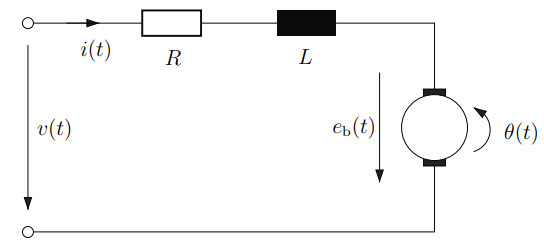
\includegraphics[width=0.6\linewidth]{figures//Results/DC_motor.png}
                \caption{DC Motor}
            \end{figure}
   \[ V(t) = L\frac{di}{dt} + R_m i(t) + K_e \omega(t) \] \\ 
     \[G(s) = \frac{21}{s(1.1s + 1)}\]

   
\end{frame}


\begin{frame}{Validation of DC Motor Learning}
     \begin{itemize}
    \item $x_1$ is the angular velocity ($\dot{\theta}$)
    \item $x_2$ is the angle ($\theta$) 
    \item control input is voltage ($v$)
    
    \end{itemize}
    \[  \dot{x} = \begin{bmatrix}
        -0.9091 & 0 \\ 
        1 & 0
    \end{bmatrix} x + \begin{bmatrix}
        4 \\ 0
    \end{bmatrix} u \] \\
   \[ y = \begin{bmatrix}
        0 & 4.7727
    \end{bmatrix} x \]

    \begin{itemize}
        \item Zoh discretization with $T_s=0.1$.
        \item initial states are $x_1 = 0$ and $x_2=\pi$
    \end{itemize}
           \[  x_{k+1} = \begin{bmatrix}
        0.9131 & 0 \\ 
        0.0956 & 1
    \end{bmatrix} x_k + \begin{bmatrix}
        0.3824 \\ 0.0194
    \end{bmatrix} u_k \] \\
     \[ yk = \begin{bmatrix}
        0 & 4.7727
    \end{bmatrix} x_k \]

%     \begin{figure}
%     \centering
%     \includesvg[width=0.6\columnwidth]{figures/DC_motor/gp_test_dc}
%     % \caption{Gaussian Process model testing of DC motor }
%     \label{fig:GP_model_testing}
    
% \end{figure}
\end{frame}

\begin{frame}{Validation of DC Motor Learning}
    \begin{figure}[!tbp]
        \centering
        \subfloat[GP model validation]{\includesvg[width=0.5\columnwidth]{figures/DC_motor/gp_test_dc}\label{fig:f1}}
        \centering
        \subfloat[Moment Matching model Validation]{\includesvg[width=0.5\columnwidth]{figures/DC_motor/long_term_test_dc}\label{fig:f1}}
    \end{figure}
%     \begin{figure}
%     \centering
%     \includesvg[width=0.8\columnwidth]{figures/DC_motor/long_term_test_dc}
%     % \caption{Longterm prediction model testing}
%     \label{fig:longterm_testing}
% \end{figure}
\end{frame}


\begin{frame}{DC Motor Without Uncertainty(Disturbances)}
    \begin{figure}[!tbp]
        \centering
        \subfloat[GP-MPC controller $t_s=8$]{\includesvg[width=0.5\columnwidth]{figures/DC_motor/gp_mpc_wo_1}\label{fig:f1}}
        \centering
        \subfloat[f-MPC controller $t_s=7$]{\includesvg[width=0.5\columnwidth]{figures/DC_motor/f_mpc_wo_dc}\label{fig:f1}}
    \end{figure}
%     \begin{figure}
%     \centering
%     \includesvg[width=0.8\columnwidth]{figures/DC_motor/gp_mpc_wo_1}
%     % \caption{GP-MPC controller- noise free DC motor plant without parameter uncertainty}
%     \label{fig:GPMPC_DC_wo_noise}
% \end{figure}
\end{frame}


\begin{frame}{DC Motor With Uncertainty(Disturbances)}
\begin{itemize}
        \item Uncertainty Model
    \end{itemize}
     \[ x_{k+1} = A_d x_k + B_d u_k + \epsilon_d \] 
    \[ A_d = A + \lambda_a A, \qquad  B_d = B + \lambda_b B \]  
    \begin{figure}[!tbp]
        \centering
        \subfloat[GP-MPC controller $t_s=11$]{\includesvg[width=0.35\columnwidth]{figures/DC_motor/mpc_dc_noise_1}\label{fig:f1}}
        \centering
        \subfloat[f-MPC controller $t_s=9$]{\includesvg[width=0.38\columnwidth]{figures/DC_motor/f_mpc_noise_1}\label{fig:f1}}
    \end{figure}
%     \begin{figure}
%     \centering
%     \includesvg[width=0.8\columnwidth]{figures/DC_motor/f_mpc_wo_dc}
%     % \caption{f-MPC controller- DC motor plant without uncertainty}
%     \label{fig:fmpc_dc_wo_noise}
% \end{figure}
\end{frame}


% \begin{frame}{Frame Title}
%     \begin{figure}
%     \centering
%     \includesvg[width=0.8\columnwidth]{figures/DC_motor/mpc_dc_noise_1}
%     % \caption{GP-MPC controller- DC motor plant with uncertainty and noisy meaurements}
%     \label{fig:Gp-mpc_noise_dc}
% \end{figure}
% \end{frame}

% \begin{frame}{Frame Title}
%     \begin{figure}
%     \centering
%     \includesvg[width=0.8\columnwidth]{figures/DC_motor/f_mpc_noise_1}
%     % \caption{f-MPC controller- DC motor plant with uncertainty and noisy measurements}
%     \label{fig:f-mpc_dc_noise}
% \end{figure}
% \end{frame}


\begin{frame}{Van der Pol Oscillator \cite{korda2020optimal}}
    \[ \frac{{d^2x}}{{dt^2}} - \mu (1 - x^2) \frac{{dx}}{{dt}} + x = 0 \]
    \begin{itemize}
        \item Exhibits limit cycle
        \item  \( \mu \) represented the damping term \( -10x_2(1 - x_2^2) \), indicating the nonlinearity and damping strength.
        \item unstable fixed point at the origin and a stable limit cycle around the origin.
        \item fourth-order Runge-Kutta (RK4) method with $T_s = 0.2$
    \end{itemize}
    
    \[         \dot{x}_1 = 2x_2 \]
      \[  \dot{x}_2 = -0.8x_1 + 2x_2 - 10x_1^2x_2 + u \]
        
\end{frame}

\begin{frame}{Phase Portrait}
%     \begin{figure}
%     \centering
%     \includesvg[width=0.6\columnwidth]{figures/vdp/phase_portrait_vector_pts}
%     % \caption{Phase portrait of the unforced Van der Pol oscillator}
%     \label{fig:pp_vdp}
% \end{figure}
    \begin{figure}
    \centering
    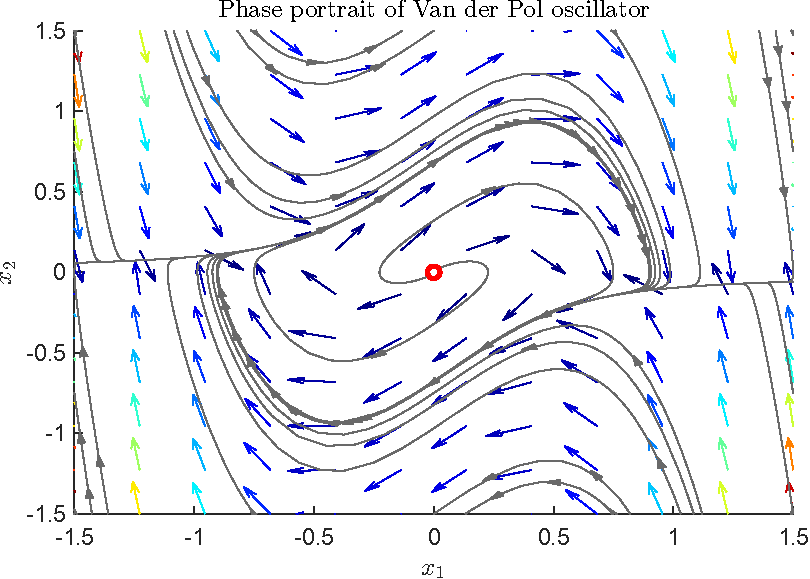
\includegraphics[width=0.6\columnwidth]{figures/vdp/phase_portarit}
    % \caption{Phase portrait of the unforced Van der Pol oscillator}
    \label{fig:pp_vdp}
\end{figure}
\end{frame}

\begin{frame}{Validation of Van der Pol Oscillator Learning}
    \begin{figure}[!tbp]
        \centering
        \subfloat[GP model validation]{\includesvg[width=0.45\columnwidth]{figures/vdp/gp_valdation_w_uncert}\label{fig:f1}}
        \centering
        \subfloat[Moment Matching model validation]{\includesvg[width=0.55\columnwidth]{figures/vdp/long_w_uncert}\label{fig:f1}}
    \end{figure}
\end{frame}


\begin{frame}{Van der Pol oscillator Without Uncertainty}
        \begin{figure}[!tbp]
        \centering
        \subfloat[GP-MPC controller $t_s=13$]{\includesvg[width=0.485\columnwidth]{figures/vdp/GP_mpc_vdp_det}\label{fig:f1}}
        \centering
        \subfloat[f-MPC controller $t_s=10$]{\includesvg[width=0.515\columnwidth]{figures/vdp/f_mpc_vdp_det}\label{fig:f1}}
    \end{figure}
\end{frame}


\begin{frame}{Van der Pol oscillator With Uncertainty}
\[\dot{x}_1 &= (2+2\lambda)x_2 \] 
        \[ \dot{x}_2 &= -(0.8+0.8 \alpha)x_1 + (2+2 \lambda)x_2 - (10+10\gamma)x_1^2x_2 + u\]
    \begin{figure}[!tbp]
        \centering
        \subfloat[GP-MPC controller $t_s=13$]{\includesvg[width=0.35\columnwidth]{figures/vdp/2_Gp_mpc_uncert_vdp}\label{fig:f1}}
        \centering
        \subfloat[f-MPC controller $t_s=9$]{\includesvg[width=0.38\columnwidth]{figures/vdp/2_f_mpc_uncert_vdp}\label{fig:f1}}
    \end{figure}
\end{frame}

\begin{frame}{Reference Tracking $x_f= [-0.25,0]$}
% \includesvg[width=0.1\columnwidth]{figures/vdp/Ref_track_pt_1}
% \includesvg[width=0.485\columnwidth]{figures/vdp/2_setpoint_gp_mpc}
% \includesvg[width=0.515\columnwidth]{figures/vdp/2_fmpc_setpont}
    \begin{figure}[!tbp]
        \subfloat{\includesvg[width=0.16\columnwidth]{figures/vdp/Ref_track_pt_1}}
        
        \subfloat[GP-MPC controller $t_s=13$]{\includesvg[width=0.35\columnwidth]{figures/vdp/2_setpoint_gp_mpc}\label{fig:f1}}
        \centering
        \subfloat[f-MPC controller $t_s=9$]{\includesvg[width=0.38\columnwidth]{figures/vdp/2_fmpc_setpont}\label{fig:f1}}
    \end{figure}
\end{frame}

\begin{frame}{Reference Tracking $x_f= [1,0]$}
        \begin{figure}[!tbp]
        \subfloat{\includesvg[width=0.16\columnwidth]{figures/vdp/phaseportatrit_2}}
        
        \subfloat[GP-MPC controller $t_s=14$]{\includesvg[width=0.38\columnwidth]{figures/vdp/5_gp_mpc_set_1_0}\label{fig:f1}}
        \centering
        \subfloat[f-MPC controller $t_s=12$]{\includesvg[width=0.4\columnwidth]{figures/vdp/5_f_mpc_set_1_0}\label{fig:f1}}
    \end{figure}
\end{frame}

% \begin{frame}{Frame Title}
    
% \end{frame}

% \begin{frame}{Frame Title}
    
% \end{frame}